\documentclass[10pt,usenames,dvipsnames]{beamer}

\usetheme{Boadilla}
\usecolortheme{crane}
\usepackage[utf8]{inputenc} 
\usepackage{graphicx}
\usepackage[french]{babel}
\usepackage{tikz}

\title{\textit{Sofware Fault Isolation} using the CompCert compiler}
\date{\today}
\author[\textit{Auteur}: Alexandre Dang \and \textit{Superviseur}: Frédéric Besson \and \textit{\'Equipe}: Celtique]
{%
	\texorpdfstring{
		\begin{columns}[t]
			\column{.45\linewidth}
				\textit{Auteur}: Alexandre Dang
			\column{.45\linewidth}
				\textit{Superviseur}: Frédéric Besson\\
				\textit{\'Equipe}: Celtique
		\end{columns}
	}
	{\textit{Auteur}: Alexandre Dang, \textit{Superviseur}: Frédéric Besson, \textit{\'Equipe}: Celtique}
}

\institute{CentraleSupélec \and %
           Université de Rennes 1
}

\AtBeginSection[]{
  \begin{frame}
  \vfill
  \centering
  \begin{beamercolorbox}[sep=8pt,center,shadow=true,rounded=true]{title}
    \usebeamerfont{title}\insertsectionhead\par%
  \end{beamercolorbox}
  \vfill
  \end{frame}
}

\setbeamertemplate{bibliography entry title}{}
\setbeamertemplate{bibliography entry location}{}
\setbeamertemplate{bibliography entry note}{}

\begin{document}
\begin{frame}
	\maketitle
\end{frame}


\begin{frame}{Flash plugin vulnérable}
	\begin{columns}[onlytextwidth]
		\begin{column}{0.5\textwidth}
			Connaissez-vous ce logo?\\
			\vspace{5mm}
			Le plugin Flash est connu pour ces failles
			$\rightarrow$~conséquences sur flash\\
			$\rightarrow$~mais AUSSI sur votre navigateur
		\end{column}
		\begin{column}{0.5\textwidth}
			\begin{figure}
				\centering
				
\includegraphics[width=0.7\textwidth]{flash.jpg}
			\end{figure}
		\end{column}
	\end{columns}
\end{frame}

\begin{frame} 
	\begin{center}{\Large Plan}\end{center}
	\tableofcontents[hideallsubsections]
\end{frame}
\section{Introduction}

\begin{frame}{Contexte}
	\begin{figure}
		\centering
		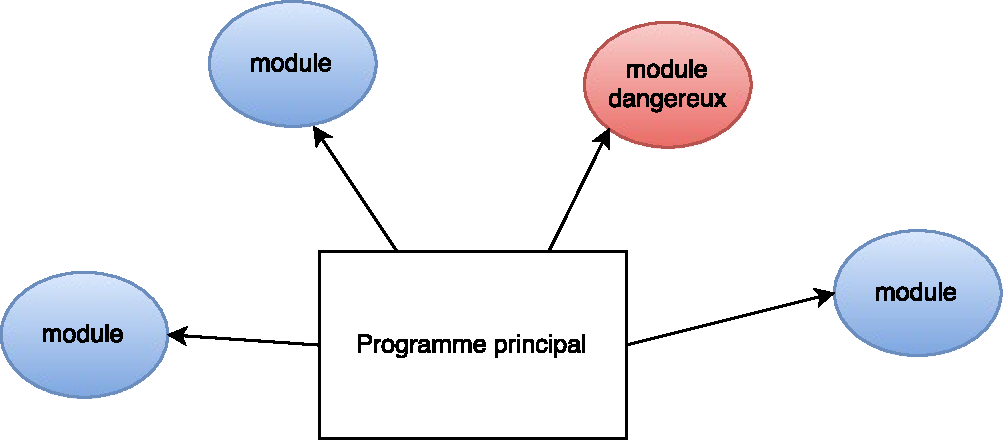
\includegraphics[width=0.7\textwidth]{module.pdf}
	\end{figure}
	\begin{itemize}
		\item les systèmes d'exploitation avec micro-noyaux
		\item un navigateur web avec ses extensions
		\item les fermes de calculs
	\end{itemize}
	
%\uncover<2>{Ces systèmes suivent un modèle commun d'un \textbf{programme} principal faisant appel à des \textbf{modules}.}
\end{frame}

\begin{frame}{Problématique}
\center{\large{Comment pouvoir exécuter ces modules potentiellement dangereux sans qu'ils puissent corrompre le programme principal?}}
\end{frame}

\begin{frame}{Solutions actuelles}
	\begin{itemize}
		\item Isolation des modules dans différents espaces mémoires
		\begin{itemize}
			\item Isolation par processus
			\item Machines virtuelles et hyperviseur
		\end{itemize}

	\alert{$\rightarrow$ les communications entre les espaces mémoires sont coûteuses en temps}
		\item \textit{Software Fault Isolation}
	\end{itemize}	
\end{frame}


\section{Fondements de Software Fault Isolation}

\begin{frame}{\textit{Software Fault Isolation}~[Wahbe et al, 1993]}
	\begin{block}{Définition}
		\textit{Software Fault Isolation} permet à un programme d'exécuter des modules dans son espace mémoire de manière sécurisée.\\
	\end{block}
	\begin{block}{Propriétés de sécurité de SFI}
		SFI garantit qu'un module respecte les propriétés suivantes:
		\begin{itemize}
			\item \textit{Sûreté de la mémoire}, le module est confiné dans une région de la mémoire appelée \textit{sandbox}
			\item \textit{Intégrité du flot de contrôle}, les interactions extérieures à la \textit{sandbox} sont contrôlées par une interface de confiance
		\end{itemize}
	\end{block}
\end{frame}

\begin{frame}{\textit{Software Fault Isolation}}
	\begin{block}{\textit{Sandbox} (bac à sable)}
		Espace contigu\"e de la mémoire où sera confiné le module à risque
		\begin{itemize}
			\item sa taille est une puissance de deux
			\item son adresse de départ est une puissance de deux
			\item identifiée par une \textbf{étiquette}
		 \end{itemize}
	\end{block}
	\center{\underline{ex}: \texttt{0xda} est l'étiquette de la \textit{sandbox} de la mémoire [\texttt{0xda000000}~-~\texttt{0xdaffffff}]}
\end{frame}

\subsection{Principes fondateurs \cite{Wahbe:1993:ESF:173668.168635}}
\begin{frame}{Composants de SFI}
	\begin{itemize}
		\item un \textbf{générateur de code}, transforme les modules afin qu'ils respectent les propriétés de SFI\\
		$\rightarrow$ hors de la \textit{Trusted Computing Base}
		\item un \textbf{vérifieur de code}, valide que le module comporte bien les transformations du générateur\\
		$\rightarrow$ fait partie de la TCB
	\end{itemize}
	\vspace{5mm}
	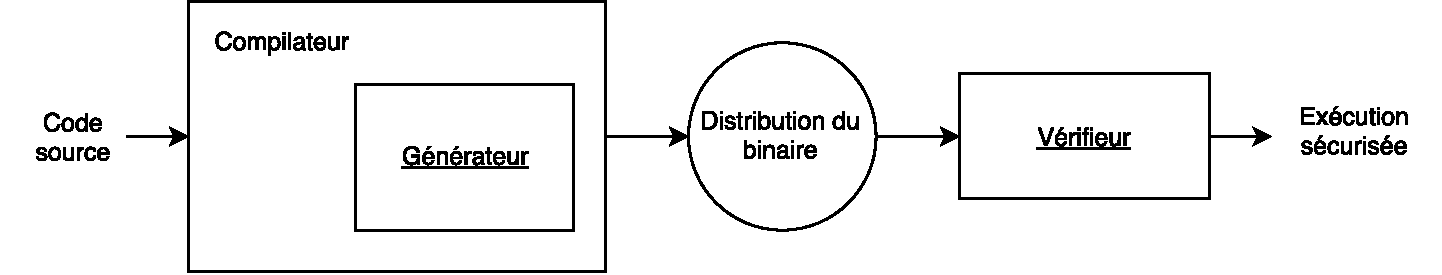
\includegraphics[width=\textwidth]{sfi_schema.pdf}
\end{frame}

%\begin{frame}{Propriétés de sécurité de SFI}
%	\begin{block}{Propriétés que doit respecter un module pour \^etre validé}
%		\begin{itemize}
%			\item \textit{Exécution fiable}, seules les instructions qui auront été analysées par le vérifieur seront exécutées
%			\item \textit{Sûreté de la mémoire}, le module à risque ne fera ni d’écriture ni de saut hors de sa \textit{sandbox} 
%			\item \textit{Intégrité du flot de contrôle}, tous les transferts de contrôle depuis les modules à risque vers le programme protégé sont identifiés et contrôlés
%		\end{itemize}
%	\end{block}
%\end{frame}

\begin{frame}{Transformations du module à risque (1/2)}
	\begin{itemize}
		\item Confinement des accès mémoire: 
		\begin{itemize}
			\item \textit{sandboxing} pour les instructions dangereuses
			\item saut dans le code (\texttt{jmp})
			\item écriture dans la mémoire (\texttt{store})
		\end{itemize}		 
			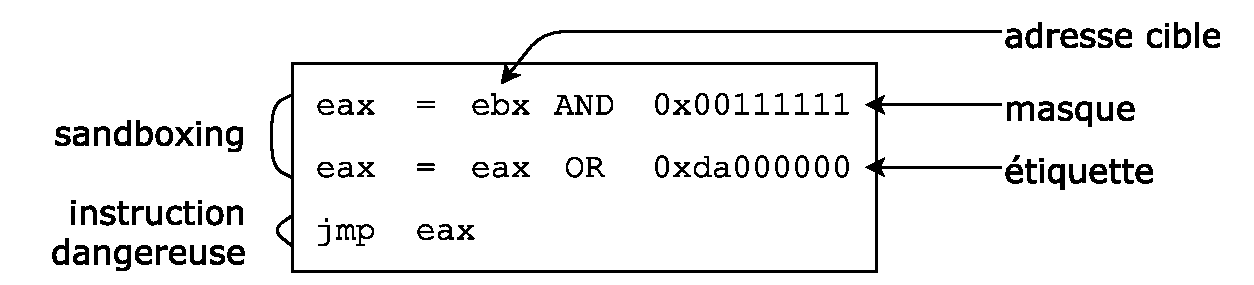
\includegraphics[scale=0.5]{algo_sandboxing.pdf}
	\end{itemize}
\end{frame}

\begin{frame}{Transformations du module à risque (2/2)}
	\begin{itemize}
		\item Contrôle des appels de fonction hors de la \textit{sandbox} via une interface de confiance faisant partie de notre TCB		
		\vspace{5mm}
		\begin{figure}
			\centering
			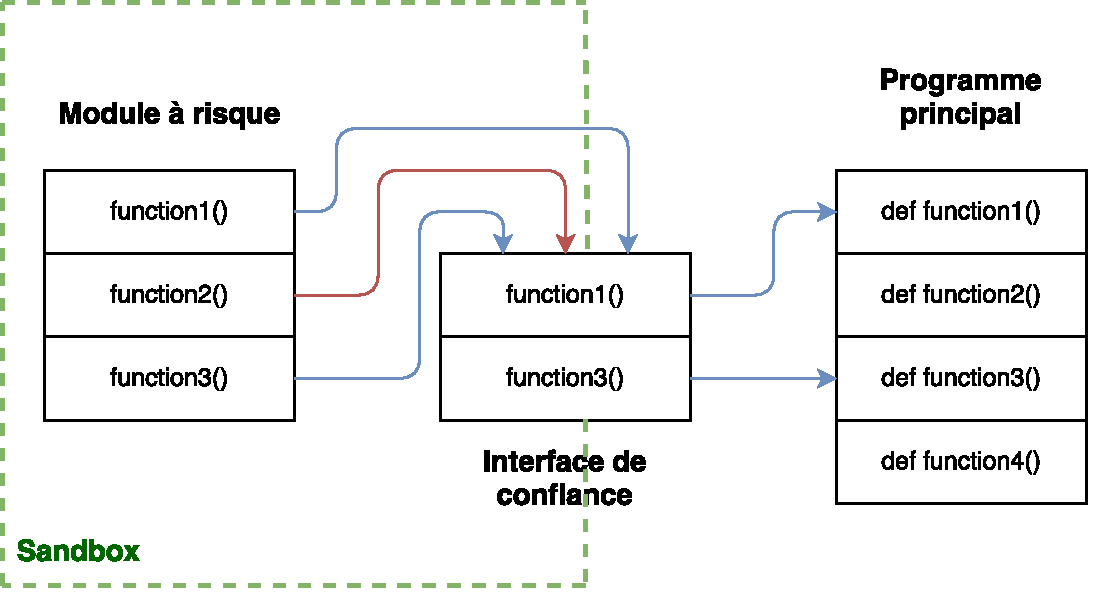
\includegraphics[width=0.85\textwidth]{interface.pdf}		
		\end{figure}
	\end{itemize}
\end{frame}

%\begin{frame}{Le vérifieur de code}
%	\begin{itemize}
%		\item fait partie de la TCB
%		\item le vérifieur valide que les transformations introduites par le générateur sont présentes et bien implémentées \\
%		$\rightarrow$ on ne peut valider que du code produit par le générateur
%	\end{itemize}
%\end{frame}

\subsection{Adaptation aux architectures modernes}
\begin{frame}{Exemple d'implémentation}
	\textbf{NativeClient}, SFI pour Google Chrome~[Yee et al, 2010][Sehr and al, 2010]
	\begin{itemize}
		\item implémentation la plus aboutie de SFI
		\item fonctionne pour les architectures x86-32, x86-64 et ARM
			\begin{itemize}
				\item jeu d'instructions différents
				\item désassemblage du binaire plus compliqué pour le vérifieur
				\item optimisations (segment mémoire physique pour x86-32, etc.)
			\end{itemize}
		\item baisses de performances de 5\% pour ARM et 7\% pour x86-64.
	\end{itemize}
\end{frame}

\begin{frame}{Avantages et inconvénients}
	\begin{itemize}
		\item Avantages
		\begin{itemize}
			\item TCB réduite au vérifieur et à l'interface de contrôle des appels externes
			\item approche indépendante du langage de programmation utilisée
		\end{itemize}
		\item Inconvénients
		\begin{itemize}
			\item le module à risque transformé est moins performant et plus lourd
			\item l'implémentation de SFI dépend de l'architecture ciblée
		\end{itemize}
	\end{itemize}
	
	\uncover<2>{\center{\alert{Est-il possible d'avoir une approche de SFI portable sur plusieurs architectures?}}}
\end{frame}

\section{Software Fault Isolation avec CompCert}
\subsection{Le compilateur certifié CompCert}
\begin{frame}{CompCert~[Leroy, 2009]}
	\begin{itemize}
		\item Compilateur certifié pour le langage C
		\item \'Ecrit et prouvé avec l'assistant à la preuve Coq
		\item Performances proches de \texttt{gcc -O1} 
	\end{itemize}
	\begin{block}{Théorème de correction de CompCert}
		Tout programme $S$ sémantiquement bien défini dans CompCert sera compilé en un code assembleur $C$ qui aura les mêmes comportements que $S$
	\end{block}
\end{frame}

\subsection{Approche SFI avec CompCert}

\begin{frame}{Approche SFI avec CompCert~[Kroll, 2014]}
	\begin{columns}
		\column{0.51\textwidth}
			{\large\underline{Objectif}: Rendre SFI portable}
			\vspace{5mm}
			\begin{itemize}
				\item transformations sur Cminor, langage indépendant de l'architecture
				\item transformations sémantiquement bien définies dans CompCert
				\item le théorème de correction de CompCert garantit que le code produit sera conforme aux exigences de SFI\\
			\end{itemize}
		\column{0.49\textwidth}
			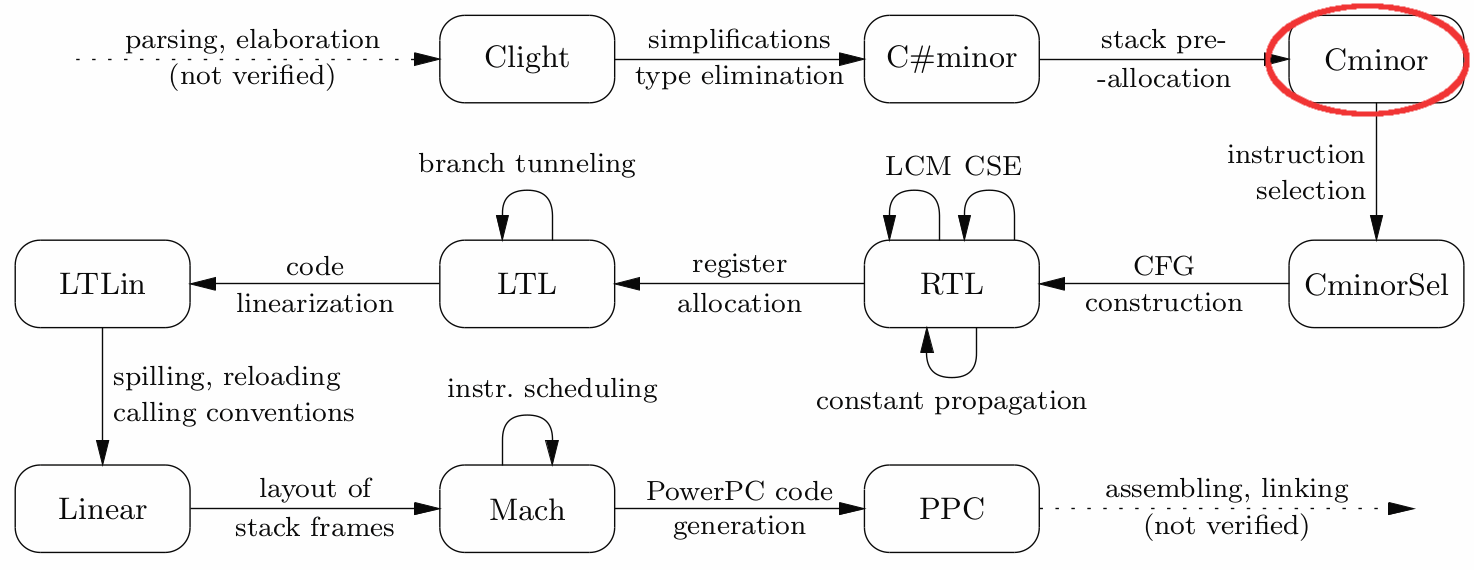
\includegraphics[width=\textwidth]{compcert_pass.png}	
	\end{columns}
	\vspace{5mm}
	$\rightarrow$ Le vérifieur de code n'est plus nécessaire dans l'approche SFI-CompCert
\end{frame}

\begin{frame}{Générateur de code avec CompCert}

	{\large SFI doit produire un code sécurisé quelque soit le programme en entrée}\\
	\vspace{5mm}
	Le Cminor transformé doit:
	\begin{enumerate}
		\item respecter les propriétés de sécurité de SFI
			\begin{itemize}
				\item opérations de \textit{sandboxing}
				\item interface de confiance pour les appels de fonction externe au module
			\end{itemize}
		\item \^etre sémantiquement défini pour que le théorème de correction s'applique
			\begin{itemize}
				\item initialisation des variables
				\item vérifications complémentaires, par exemple contre la division par 0
			\end{itemize}
	\end{enumerate}
\end{frame}

\begin{frame}{\'Evaluation de l'approche}
	\begin{itemize}
		\item Avantages
			\begin{itemize}
				\item portabilité sur toutes les architectures supportées par CompCert
				\item les transformations sur Cminor  peuvent être optimiser durant la compilation
				%\item on soustrait de la TCB le vérifieur et on rajoute les opérations non certifiés dans CompCert****
			\end{itemize}
		\item Inconvénients
			\begin{itemize}
				\item CompCert n'a pas de sémantique pour les programmes  multi-tâches
				\item la distribution des binaires n'est plus possible
			\end{itemize}
		\item Performances
			\begin{itemize}
				\item compromis entre \texttt{gcc -O0} et \texttt{gcc -O1}
				\item baisse des performances de 21,7\% sur x86 et 16,8\% sur ARM par rapport à CompCert sans SFI
			\end{itemize}
	\end{itemize}
\end{frame}

\section{Conclusion}

\begin{frame}{Conclusion}
	\begin{itemize}
		\item SFI permet d'exécuter un module à risque de manière sécurisée en:
		\begin{itemize}
			\item confinant ses accès mémoires dans la \textit{sandbox}
			\item contrôlant les appels de fonctions externes
		\end{itemize}
		\item Deux approches possibles:
		\begin{itemize}
			\item approche classique avec générateur de code et vérifieur de confiance
			\item générateur de code avec le compilateur CompCert
		\end{itemize}
	\end{itemize}
\end{frame}

\begin{frame}{Problématique du stage}
	\begin{itemize}
		\item \texttt{ret} n'utilise pas de registres pour l'adresse de retour	
		%\item SFI ne protège pas d'une réécriture dans la pile (\textit{buffer overflow})
		\item impossible de sécuriser par une opération de masquage dans la \textit{sandbox}
		\item solution utilisée:
	\end{itemize}
	\begin{figure}
		\centering
		
\includegraphics[scale=0.17]{ret_pop.png}	
	\end{figure}
	\uncover<2>{\center{\large{\alert{Les architectures modernes ont de nombreuses optimisations liées à l'instruction \texttt{ret}}}}}
\end{frame}

\begin{frame}{Approche proposée}
	\begin{columns}
		\column{.67\textwidth}
			\begin{itemize}
				\item Objectifs
					\begin{itemize}
						\item intégrité du flot de contrôle des instructions \texttt{ret}
						\item gains en performances
						\item utiliser le compilateur CompCert
					\end{itemize}
				\item<2-> Idée
					\begin{itemize}
						\item pile avec des trames de taille constante\\
						$\rightarrow$ protection des adresses de retour\\
						$\rightarrow$ protection contre les attaques de type \textit{buffer overflow}
					\end{itemize}
				\item<3> Difficultés envisagées
					\begin{itemize}
						\item choix d'un niveau de langage pour implémenter les transformations SFI
						\item langage haut niveau comme Cminor, nécessite de définir une sémantique à nos transformations dans la chaîne de compilation
						\item langage bas niveau implémentation plus complexe
					\end{itemize}
			\end{itemize}
		\column{.3\textwidth}
			\uncover<2->{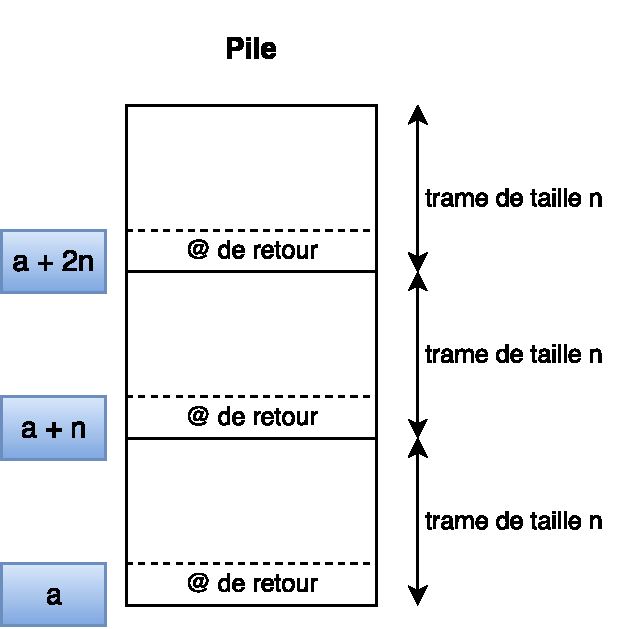
\includegraphics[width=\textwidth]{pile.pdf}}
	\end{columns}
\end{frame}

\begin{frame}{Fin}
	\center{\huge{Merci de votre attention}}
\end{frame}

\nocite{Kroll:2014:PSF:2708449.2708686}
\nocite{Leroy:2009:FVR:1538788.1538814}
\nocite{Sehr:2010:ASF:1929820.1929822}
\nocite{Wahbe:1993:ESF:173668.168635}
\nocite{Yee:2010:NCS:1629175.1629203}
\nocite{Abadi:2009:CIP:1609956.1609960}
\nocite{Mccamant_evaluatingsfi}
\nocite{compCert_memory_model}
\nocite{Zeng:2011:CCI:2046707.2046713}

\begin{frame}[noframenumbering]{References}
	\scriptsize
	\setbeamertemplate{bibliography item}{\insertbiblabel}
	\bibliographystyle{plain}
    \bibliography{ref}
\end{frame}
\end{document}

%jeu d'instructions plus complexes, désassemblage, segments mémoire x86-32
%TCB réduite, générateur certifié ...
%Expliquer les perfs sont pourries, montrer que y a des opt encore, prototype de recherche et qu'il pourrai faire beaucoup mieux
%Faire une conclusion qui ouvre sur notre recherche et dire qu'on va utiliser CompCert
%schéma pile de taille constatnte
